\section{A roofline for reclamation policy}
\label{sec:roofline}

The previous sections describe \emph{what} the mechanism does.
This section answers the question a user actually asks when choosing knobs: given a memory budget and a
pause budget, what is the cheapest policy, and how much does each megabyte buy?
We borrow the shape of the GPU roofline model \cite{williams2009roofline} because the structure of the
problem is the same: an application has a \emph{rate} (bytes allocated per second) and a \emph{cost
per unit of work} (nanoseconds of collector time per byte reclaimed), and the two are linked by a
machine roof and by two walls.
The difference is that the GPU's walls are hardware constants while ours are \emph{contract}
parameters, which is what makes the model a policy tool rather than a measurement plot.

\subsection{The analogy, item by item}
\label{sec:roofline-analogy}

\begin{table*}[t]
\centering
\small
\resizebox{\ifdim\width>\linewidth\linewidth\else\width\fi}{!}{\begin{tabular}{@{}lll@{}}
\toprule
GPU roofline & Reclamation roofline & Form \\
\midrule
arithmetic intensity $I = \mathit{FLOP}/\mathit{Byte}$ & reclamation intensity $1/\lambda$ & bytes reclaimed per ns of collector time \\
peak compute $\pi$ & compute roof $\rho/\lambda$ & $a \le \rho/\lambda$, $\rho = 1$ (serial on the mutator thread) \\
memory bandwidth $\beta$ & mutator platform $a_{\text{peak}}$ & $a \le a_{\text{peak}}$; measured $\ge 10.2$\,GB/s \\
ridge point $I^{\ast} = \pi/\beta$ & ridge $\lambda^{\ast} = \rho/a_{\text{peak}}$ & $a_{\text{peak}} = 10.2$\,GB/s $\Rightarrow \lambda^{\ast} = 0.098$\,ns/B \\
two walls (compute, bandwidth) & two walls (memory, pause) & $r \le r_{\max}(M_{\max})$, $b \le b_{\max}(P_{\max})$ \\
point below the roof & point far below the platform & \S\ref{sec:roofline-plane}: extC sits $33\times$ below \\
\bottomrule
\end{tabular}}
\caption{The analogy, item by item. The only structural difference is that both walls are contract
parameters set by the user rather than hardware constants.}
\label{tab:roofline-map}
\end{table*}

The mapping is not decorative: it says which quantity to optimize.
In the GPU model one raises arithmetic intensity until the kernel hits the compute roof.
Here one raises $1/\lambda$ -- that is, lowers the cost of reclaiming a byte -- until the collector
stops being the roof, and then chooses the two ratio knobs so that the program sits inside the
feasible window rather than against a wall.

\subsection{The cost model}
\label{sec:roofline-cost}

Fix a region and consider one collection round.
Let $L$ be the live bytes at the trigger and $H = rL$ the heap at the trigger, so $r = H/L$ is the
\emph{retention ratio} and $\sigma = 1/r$ the \emph{liveness fraction}.
Let $b$ be the batch: the maximum number of objects a mark step may pop
(\texttt{MARK\_BATCH\_MAX}, 256).
Let $K$ be the number of allocations after which the mechanism may make one unit of reclamation
progress (\texttt{MARK\_EVERY}, 64), and $g$ the average number of pushes per marked object ($2.76$
on our shapes).
The calibration of \S\ref{sec:roofline-calib} gives $c_t = 0.4114$\,ns per live byte traced,
$c_s = 0.0108$\,ns per heap byte swept, $F_{\text{slab}} = 1.30$ (slab bytes touched per live byte,
from fragmentation), $\tau_t = 17.49$\,ns per marked object and $\tau_s = 0.458$\,ns per freed slot.

\begin{theorem}[Cost law]
\label{thm:cost}
For $r > 1$ the amortized reclamation cost per allocated byte is
\begin{equation}
\label{eq:lambda}
\lambda(r) = \frac{c_t + c_s F_{\text{slab}}\, r}{r - 1}
= c_s F_{\text{slab}} + \frac{c_t + c_s F_{\text{slab}}}{r-1},
\end{equation}
which is strictly decreasing in $r$ with infimum $c_s F_{\text{slab}}$, and independent of $b$.
\end{theorem}
\begin{proof}
A round reclaims $(r-1)L$ bytes.
Marking visits every live object, at cost $c_t L$ (the per-object fixed cost $\tau_t/\bar{s}$ is
absorbed into $c_t$).
Sweeping covers the slab bytes of the region, at cost $c_s F_{\text{slab}}\, rL$.
Dividing the sum by the reclaimed bytes gives eq.~\ref{eq:lambda}; the derivative is
$-(c_t + c_s F_{\text{slab}})/(r-1)^2 < 0$ and the limit is the floor.
The batch $b$ bounds how much work one step performs, not how much a round performs, so it does not
appear.
\end{proof}

\begin{theorem}[Memory law]
\label{thm:memlaw}
At a trigger, resident bytes are $M = L + \kappa_M\,H + O(B)$ with
$\kappa_M \in [0.772, 1.010]$, hence
\begin{equation}
\begin{aligned}
M_{\text{peak}} &\le L\,(1 + \kappa_M\, r_{\max}),\\
r_{\max}(M_{\max}) &= \frac{M_{\max}/L - 1}{\kappa_M}.
\end{aligned}
\label{eq:memlaw}
\end{equation}
\end{theorem}
\begin{proof}[Proof sketch]
The retained set at a trigger is the live set plus garbage the credit rule has not yet allowed to be
traversed; the credit rule admits $\max(2L, G)$ unvisited bytes, which is what makes $\kappa_M$ a
constant rather than a function of history (\thm\ref{thm:mem}).
The $O(B)$ term is one slab of quantization.
\end{proof}

\begin{theorem}[Pause law]
\label{thm:pauselaw}
A mark step taking batch $b$ costs
\begin{equation}
\label{eq:pauselaw}
P(b) = b\,\tau_t + W_s \cdot 64 \cdot \tau_s + c_0
= 17.49\,b + 234.5\text{ ns} + c_0,
\end{equation}
with $W_s = 8$ words of sweep per step and $c_0$ the fixed step overhead; at $b = 256$ this is
$4.71$\,\us.
\end{theorem}
\begin{proof}[Proof sketch]
A step pops at most $b$ objects and pays $\tau_t$ per pop for descriptor dispatch and child pushes;
a sweep step visits at most $W_s$ bitmap words and frees at most $64 W_s$ slots at $\tau_s$ each.
The segment restart cost is charged to $c_0$; \thm\ref{thm:pause} states the full bound including the
segment deadline.
\end{proof}

\begin{theorem}[Keep-up law]
\label{thm:keepup}
A policy with batch $b$ keeps up with the mutator only if
\begin{equation}
\label{eq:keepup}
\sigma \le \frac{b}{b + gK}
\quad\Longleftrightarrow\quad
r \ge r_{\min}(b) = 1 + \frac{gK}{b}.
\end{equation}
\end{theorem}
\begin{proof}[Proof sketch]
Let the mutator allocate $H = rL$ bytes per round, i.e. $rL/\bar{s}$ objects; reclamation must retire
the same number of slots per round to keep $H$ constant.
The progress budget allows one unit of work per $K$ allocations and $b$ objects per step, and the
factor $g$ converts marked objects into pushes, so the reclamation side advances $b/(gK)$ slots per
allocated slot.
Requiring that advance to be at least one gives eq.~\ref{eq:keepup}.
Both extremes check out: $b \to \infty$ gives $r_{\min} \to 1$ (unlimited budget can always catch
up) and $g = 0$ gives $r_{\min} \to 1$ (no children to trace).
\end{proof}

The two laws create the tension that the rest of this section resolves.
\thm\ref{thm:cost} wants $r$ large, \thm\ref{thm:memlaw} caps $r$ at $r_{\max}(M_{\max})$, and
\thm\ref{thm:keepup} forbids $r$ below $r_{\min}(b)$ -- while raising $b$ tightens the pause ceiling
of \thm\ref{thm:pauselaw} but \emph{lowers} $r_{\min}$.
The policy problem is the placement of $r$ inside $[r_{\min}(b), r_{\max}]$ with $b$ as large as the
pause budget allows.

\subsection{The feasible window}
\label{sec:roofline-feasible}

\begin{theorem}[Feasibility]
\label{thm:feasible}
Given a memory budget $M_{\max}$ and a pause budget $P_{\max}$, a policy $(b, r)$ meeting both
contracts exists if and only if
\begin{equation}
\begin{aligned}
\&\lambda_{\min}(M_{\max}) \le \lambda_{\text{keep}}(b_{\max}(P_{\max}))\\
\&\quad\Longleftrightarrow\quad M_{\max} \ge L\,(1 + \kappa_M\, r_{\min}(b_{\max})),
\end{aligned}
\label{eq:feasible}
\end{equation}
where $\lambda_{\min}(M_{\max}) = \lambda(r_{\max})$ and
$\lambda_{\text{keep}}(b) = \lambda(r_{\min}(b))$.
\end{theorem}
\begin{proof}[Proof sketch]
$\lambda$ decreases by \thm\ref{thm:cost}, so the memory contract forces
$\lambda \ge \lambda(r_{\max})$, and keep-up forces $r \ge r_{\min}(b)$, i.e.
$\lambda \le \lambda(r_{\min}(b))$.
A ratio exists in the interval exactly when the two bounds do not cross, which is eq.~\ref{eq:feasible};
substituting eq.~\ref{eq:memlaw} turns it into the memory form.
\end{proof}

\begin{corollary}
\label{cor:floor}
There is a minimum feasible heap $M_{\min} = L\,(1 + \kappa_M\,r_{\min}(b))$ -- $6.28$\,MB for a
$2.333$\,MB live set with $b = 256$ and $\kappa_M = 1$.
Below it no choice of knobs satisfies both contracts; the escapes are a cheaper collector, a smaller
live set, or a weaker contract.
\end{corollary}

This corollary is the model's main practical value: it tells a user, before running the program,
whether a memory target is reachable at all.

\subsection{The optimal policy is a corner}
\label{sec:roofline-optimal}

\begin{theorem}[Optimality]
\label{thm:optimal}
Inside the feasible window the tax is minimized at
\begin{equation}
\begin{aligned}
b^{\ast} &= \min\left(256, \left\lfloor \frac{P_{\max} - W_s\cdot 64\cdot\tau_s}{\tau_t} \right\rfloor\right),\\
r^{\ast} &= \frac{M_{\max}/L - 1}{\kappa_M},
\end{aligned}
\end{equation}
with per-byte cost $\lambda^{\ast} = \lambda(r^{\ast} + 0.4)$, where $+0.4$ is the measured offset
between the peak-round ratio and the effective ratio over a whole run.
The resulting collection tax is $\lambda^{\ast} a/(1 + \lambda^{\ast} a)$ at mutator allocation rate
$a$, and the achieved throughput is $a_{\text{all}} = a/(1 + \lambda^{\ast} a)$.
\end{theorem}
\begin{proof}[Proof sketch]
$\lambda$ decreases in $r$, so the objective is minimized by the largest feasible $r$, which the memory
contract caps at $r_{\max}$; $r_{\min}$ decreases in $b$, so the largest allowed batch is best and it
also relaxes eq.~\ref{eq:pauselaw}.
Both knobs sit at their walls: memory decides the retention ratio, the pause budget decides the batch.
The tax formula is the serial-fraction identity: per unit of mutator work the collector adds
$\lambda^{\ast}$ ns per allocated byte, and the mutator allocates $a$ bytes per ns.
\end{proof}

\begin{proposition}[Ridge]
\label{prop:ridge}
The collector stops being the roof when $\lambda^{\ast} \le \rho/a_{\text{peak}}$, i.e.
$\lambda^{\ast} \le 0.098$\,ns/B for a $10.2$\,GB/s platform.
Above that intensity the program is \emph{reclamation-limited}; below it, mutator-limited.
\end{proposition}

\subsection{The plane}
\label{sec:roofline-plane}

\begin{figure}[t]
\centering
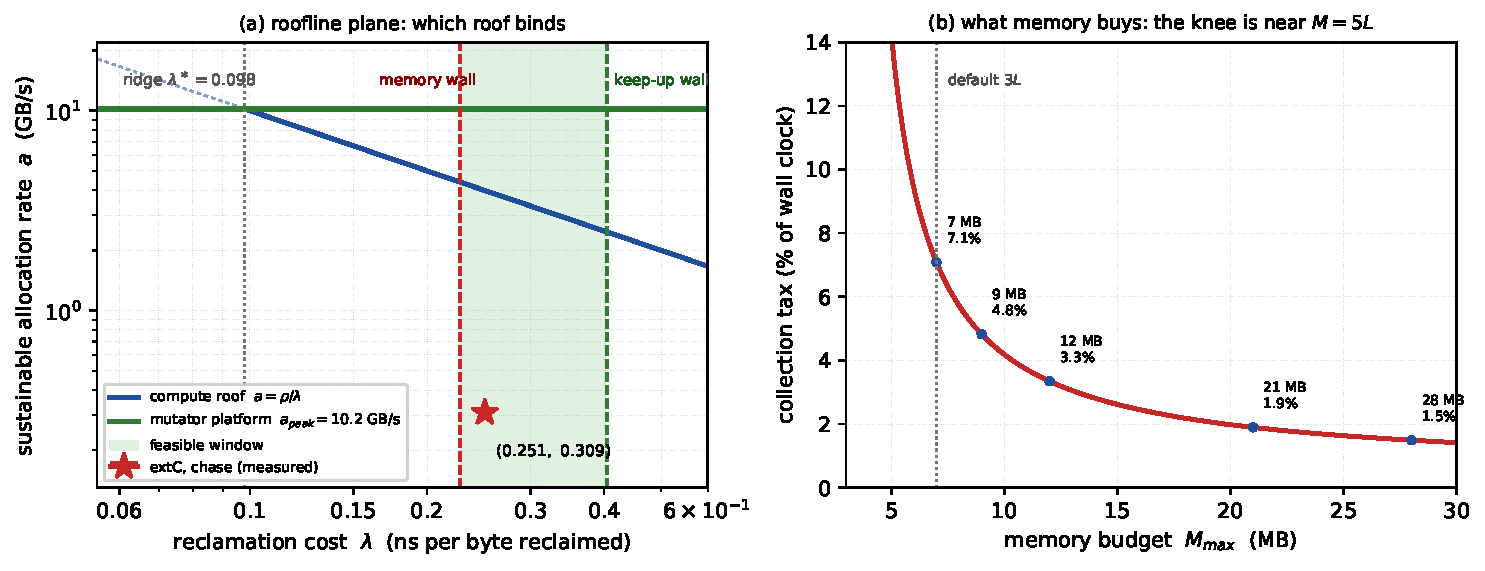
\includegraphics[width=0.95\linewidth]{figures/roofline.pdf}
\caption{The reclamation roofline for a $2.333$\,MB live set and the measured constants
(\tab\ref{tab:calib}).
(a) Horizontal: the mutator platform $a_{\text{peak}} = 10.2$\,GB/s; curved: the compute roof
$a = \rho/\lambda$, dotted where it lies above the platform and therefore does not bind.
Shaded: the feasible window between the two dashed walls, for $M_{\max} = 7$\,MB and
$P_{\max} = 5$\,\us -- outside it no knob setting meets both contracts.
The star is the measured working point on the pointer-chasing shape.
(b) The same model against the memory budget: collection tax at $a = 0.335$\,GB/s, with the knee
near $M = 5L$ (\tab\ref{tab:pareto}).}
\label{fig:roofline}
\end{figure}

\fig\ref{fig:roofline} is the whole model in one picture.
The ordinate is the allocation rate a workload can sustain; the abscissa is the cost of reclaiming a
byte.
A policy moves vertically only by becoming cheaper per byte (lower $\lambda$), and horizontally only by
spending memory, since lower $\lambda$ needs higher $r$ and $r$ is capped by $M_{\max}$.
The two vertical walls are the contracts: left of $\lambda_{\text{keep}}$ the collector cannot keep up
with the mutator; right of $\lambda_{\min}$ the program exceeds its memory budget.

\paragraph{Where extC sits.}
For the pointer-chasing shape of \S\ref{sec:eval} the measured working point is
$\lambda = 0.2508$\,ns/B at $a_{\text{all}} = 0.309$\,GB/s -- a factor $33$ below the platform, i.e.
deep in the mutator-limited region, which matches the $3.9\%$ collection share that \S\ref{sec:eval}
reports for that shape.
On the allocation-heavy shapes the same policy sits at the other end, where the tax is a large
fraction of the wall clock and improving $\lambda$ pays.

\subsection{What memory buys}
\label{sec:roofline-pareto}

\begin{table*}[t]
\centering
\small
\resizebox{\ifdim\width>\linewidth\linewidth\else\width\fi}{!}{\begin{tabular}{@{}rrrrrr@{}}
\toprule
$M_{\max}$ & $r_{\max}$ (typ.) & $r_{\max}$ (cons.) & $r_{\text{eff}}$ & $\lambda^{\ast}$ (ns/B) & tax \\
\midrule
 7\,MB (default $3L$) & 2.59 & 2.00 & 2.99 & 0.2277 & 7.1\% \\
 9\,MB & 3.70 & 2.86 & 4.10 & 0.1512 & 4.8\% \\
12\,MB & 5.37 & 4.14 & 5.77 & 0.1033 & 3.3\% \\
21\,MB & 10.36 & 8.00 & 10.76 & 0.0576 & 1.9\% \\
28\,MB & 14.25 & 11.00 & 14.65 & 0.0452 & 1.5\% \\
$\infty$ (floor) & -- & -- & $\infty$ & 0.0140 & 0.47\% \\
\bottomrule
\end{tabular}}
\caption{Pareto front of tax against memory, from eqs.~\ref{eq:lambda}--\ref{eq:memlaw} at
$L = 2.333$\,MB, $a = 0.335$\,GB/s and $b = 256$; ``typ.'' uses the measured $\kappa_M = 0.772$,
``cons.'' the conservative $\kappa_M = 1$ that the contract assumes. Regenerated by
\texttt{figures/gen\_roofline.py}.}
\label{tab:pareto}
\end{table*}

\tab\ref{tab:pareto} answers the question users ask most often: how much memory should I give the
collector?
The marginal return decays quickly.
Going from the default $3L$ to $12$\,MB cuts the tax from $7.1\%$ to $3.3\%$; from $12$ to $21$\,MB
takes it to $1.9\%$; beyond $21$\,MB each additional megabyte buys less than $0.1$ percentage point,
because the floor of eq.~\ref{eq:lambda} is approached as $1/r$.
The memory wall is therefore a knee rather than a wall, and for our constants the knee sits near
$M = 5L$.

\subsection{Calibration}
\label{sec:roofline-calib}

\begin{table*}[t]
\centering
\small
\resizebox{\ifdim\width>\linewidth\linewidth\else\width\fi}{!}{\begin{tabular}{@{}llrl@{}}
\toprule
Constant & Meaning & Value & Accuracy \\
\midrule
$c_t$ & tracing cost per live byte & 0.4114\,ns/B & $\pm 2\%$ (two shapes) \\
$c_s F_{\text{slab}}$ & sweep floor per heap byte & 0.01404\,ns/B & $\pm 1\%$ \\
$F_{\text{slab}}$ & slab bytes per live byte & 1.30 & measured \\
$\kappa_M$ & retained garbage per live byte & 0.772 / 0.825 / 1.010 & three shapes \\
$\tau_t$ & trace cost per object & 17.49\,ns & $\pm 5\%$ \\
$\tau_s$ & sweep cost per freed slot & 0.458\,ns & $\pm 10\%$ \\
$g$ & pushes per marked object & 2.76 & uncertain, $\le 5.7$ \\
$K$ & allocations per progress unit & 64 & compile-time constant \\
$\rho$ & serial-fraction coefficient & 1 & by construction \\
\bottomrule
\end{tabular}}
\caption{Calibrated constants. The $c_s$ floor and the $\tau_s$ worst case are different
measurements -- the first is amortized over whole-dead-slab elision, the second is the per-slot cost
when slots must actually be freed -- which is why $c_s\cdot 16 < \tau_s$.}
\label{tab:calib}
\end{table*}

\tab\ref{tab:calib} lists every constant the model uses.
Equations~\ref{eq:lambda}--\ref{eq:pauselaw} reproduce the measured per-byte costs to within
$2$--$10\%$ at the calibrated shapes, the same order as the run-to-run drift of the machine;
model predictions are therefore quoted to two significant digits and never used to decide differences
smaller than that.
Two constants carry the model uncertainty: $g$ comes from a structural count on an older revision
($\le 5.7$ at the outside, which moves $r_{\min}$ by $1.4\times$), and $\tau_t$ varies by shape
because descriptor dispatch differs.

\subsection{Using the model}
\label{sec:roofline-use}

The model is used in three ways in this paper, and only the third is post hoc.

\paragraph{Entering the window.}
For a new workload we measure $L$ and $a$, then ask whether the default $M_{\max} = 3L$ is above
$M_{\min}$ (\cor\ref{cor:floor}).
For the pointer-chasing shape it is -- $6.28$\,MB of floor against $7$\,MB, a $1.11\times$ margin --
which is why that shape is the one where the collection share is a few percent.

\paragraph{Choosing the knobs.}
\thm\ref{thm:optimal} fixes $b$ from the pause budget and $r$ from the memory budget.
extC's defaults are the contract corner with $b = 256$ and the implicit $M_{\max} = 3L$; a user who
wants a $50$\,\us pause budget keeps $b = 256$ because $4.71$\,\us fits, and the compile-time cap of
$256$ exists because larger batches change the pressure multiplier rather than the steady-state
pause.

\paragraph{Explaining a measurement.}
When a shape is slower than its competitor the model decomposes the difference into a $\lambda$ term
and a non-$\lambda$ term.
For the pointer-chasing shape that decomposition attributes $3.9\%$ of the wall clock to collection
and $1.9\%$ to cache-line phase conflicts between 48-byte slots and 64-byte lines -- a layout effect
the model does not describe, which is why it is reported separately instead of folded into
$\lambda$.

\subsection{What the model does not claim}
\label{sec:roofline-limits}

Four boundaries of the model are worth stating.
(i) It is a \emph{single-threaded, single-region} model; it says nothing about per-task arenas or
parallel workers, where the bound becomes a sum over arenas.
(ii) $\lambda$ assumes a full mark per round; the chunked implementation performs the same total work
but distributes it, so $\lambda$ bounds the tax and \thm\ref{thm:pause} bounds the pause, and neither
bounds the other.
(iii) $\kappa_M$ is calibrated on shapes with uniform garbage; a shape that interleaves a long-lived
mutable structure with a short-lived one can exceed it, which is why the contract uses the
conservative $\kappa_M = 1$ and the measurements report the typical value.
(iv) The model prices \emph{reclamation} only.
Allocation itself costs instructions, and on the allocation-heavy shapes that fixed cost is
comparable to the collection tax; it is measured separately (\S\ref{sec:eval}) rather than hidden in
$\lambda$.